% Appendix B — Allen-Dynes strong-coupling Tc. Filled standalone, \input'd by main.tex.
\section{Allen--Dynes $T_c$ (Strong Coupling)}
\label{app:allendynes}

This appendix is the full data record for the Allen--Dynes
\citep{allendynes1975} strong-coupling refinement --- pipeline stage
\textcircled{\scriptsize 3} for $\lambda\!\gtrsim\!1.5$, the regime the
hydride candidates of Appendix~\ref{app:hydride} occupy. It states the
$f_1$ (strong-coupling) and $f_2$ (spectral-shape) correction factors of
Eq.~\eqref{eq:allendynes} verbatim, including $\Lambda_1$, $\Lambda_2$,
and the $\bar\omega_2/\omega_{\log}$ ratio, and records the headline
recompute (h3cl: $\texttt{allen\_dynes\_tc}\!=\!140.324$\,K,
$|\Delta|\!=\!2.8\!\times\!10^{-11}$, V3 ledger). Data sources: the
\texttt{allen\_dynes\_tc} atom in \texttt{companion/verify-ledger.json}.

% -------------------------------------------------------------------------
\subsection{The strong-coupling form}
\label{app:ad-eq}

Allen and Dynes \citep{allendynes1975} relaxed McMillan's fixed-spectral-
shape assumption by multiplying the McMillan exponential by two correction
factors $f_1$ (strong-coupling) and $f_2$ (spectral-shape):
\begin{equation}
T_c \;=\; \frac{f_1\,f_2\,\omega_{\log}}{1.20}\,
  \exp\!\left[-\,\frac{1.04\,(1+\lambda)}
                     {\lambda - \mu^{*}\,(1+0.62\,\lambda)}\right].
\label{eq:ad-app}
\end{equation}
The two factors are themselves closed forms of $\lambda$, $\mu^{*}$, and
the spectral ratio $\bar\omega_2/\omega_{\log}$:
\begin{align}
f_1 &\;=\; \left[\,1 + \left(\frac{\lambda}{\Lambda_1}\right)^{3/2}\,\right]^{1/3},
   & \Lambda_1 &\;=\; 2.46\,(1 + 3.8\,\mu^{*}),
   \label{eq:f1}\\[4pt]
f_2 &\;=\; 1 + \frac
   {\big[(\bar\omega_2/\omega_{\log}) - 1\big]\,\lambda^2}
   {\lambda^2 + \Lambda_2^2},
   & \Lambda_2 &\;=\; 1.82\,(1 + 6.3\,\mu^{*})\,\frac{\bar\omega_2}{\omega_{\log}}.
   \label{eq:f2}
\end{align}
Here $\bar\omega_2=\big[(2/\lambda)\!\int\!\omega\,\alpha^2F\,d\omega\big]^{1/2}$
is the second (mean-square) spectral moment and $\omega_{\log}$ the
logarithmic moment (Appendix~\ref{app:elph}). $f_1$ \emph{lifts} $T_c$ at
strong coupling --- it grows without bound as $\lambda\!\to\!\infty$,
$f_1\!\sim\!(\lambda/\Lambda_1)^{1/2}$, recovering the
Allen--Dynes $T_c\!\propto\!\sqrt{\lambda}\,\omega_{\log}$ asymptote that
McMillan lacks. $f_2$ corrects for the \emph{shape} of $\alpha^2F$: a
broad spectrum ($\bar\omega_2/\omega_{\log}\!>\!1$) raises $T_c$, a peaked
one lowers it; $f_2\!=\!1$ when $\bar\omega_2=\omega_{\log}$ (a single
Einstein mode) or when $\lambda\!\to\!0$.

% -------------------------------------------------------------------------
\subsection{Strong-coupling enhancement curve}
\label{app:ad-enhance}

The physically meaningful quantity is the \emph{enhancement} $f_1 f_2$
over the McMillan exponential. Fig.~\ref{fig:ad-enhance} plots $f_1$ (the
$f_2$-neutral enhancement) vs $\lambda$ at $\mu^{*}=0.10$: it is unity at
weak coupling (Allen--Dynes $\to$ McMillan, the consistency check) and
rises past $1.4$ by $\lambda=3.4$ (the CaH$_6$ regime), which is the
$\sim\!40$\% lift that closes the McMillan under-prediction of
Appendix~\ref{app:mcmillan}.

\begin{figure}[h]
\centering
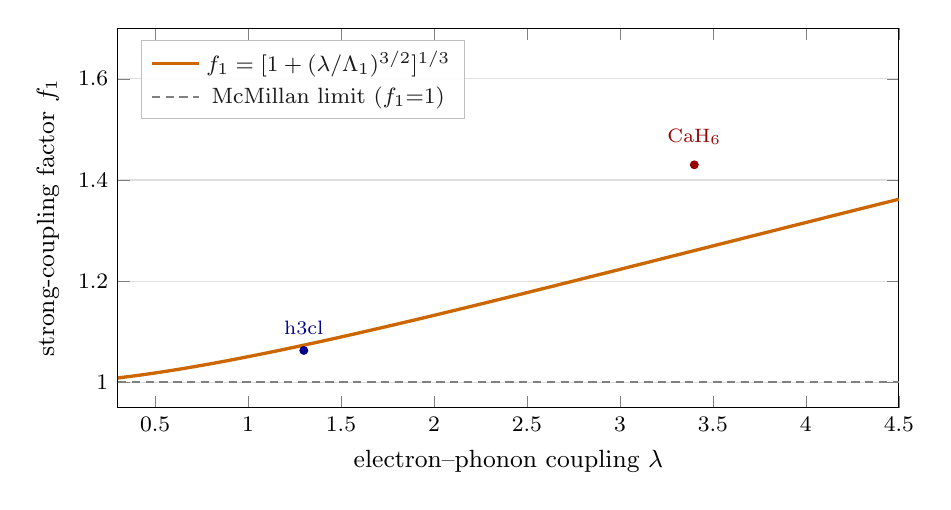
\begin{tikzpicture}
\begin{axis}[
  width=11.5cm, height=6.4cm,
  xlabel={electron--phonon coupling $\lambda$},
  ylabel={strong-coupling factor $f_1$},
  xmin=0.3, xmax=4.5, ymin=0.95, ymax=1.7,
  tick label style={font=\footnotesize},
  label style={font=\small},
  ymajorgrids, grid style={gray!25},
  domain=0.3:4.5, samples=80,
  legend pos=north west,
  legend style={font=\footnotesize,fill=white,fill opacity=0.9,draw=gray!50},
]
\addplot[orange!80!black,very thick,smooth]
  {(1+(x/(2.46*(1+3.8*0.10)))^1.5)^(1/3)};
\addlegendentry{$f_1=[1+(\lambda/\Lambda_1)^{3/2}]^{1/3}$}
\addplot[gray,densely dashed,thick] {1};
\addlegendentry{McMillan limit ($f_1{=}1$)}
% candidate markers
\node[font=\scriptsize,blue!55!black,anchor=south] at (axis cs:1.30,1.075) {h3cl};
\draw[blue!55!black,fill=blue!55!black] (axis cs:1.30,1.063) circle (1.4pt);
\node[font=\scriptsize,red!60!black,anchor=south] at (axis cs:3.40,1.45) {CaH$_6$};
\draw[red!60!black,fill=red!60!black] (axis cs:3.40,1.43) circle (1.4pt);
\end{axis}
\end{tikzpicture}
\caption{Allen--Dynes strong-coupling factor $f_1$ vs $\lambda$ at
$\mu^{*}=0.10$ (Eq.~\ref{eq:f1}). $f_1\!\to\!1$ at weak coupling (the
Allen--Dynes\,$\to$\,McMillan consistency limit) and rises to $\sim\!1.43$
at the CaH$_6$ coupling $\lambda=3.4$ --- this lift is precisely the
fraction by which McMillan under-predicts $T_c$ in the high-$\lambda$
hydride regime (Appendix~\ref{app:mcmillan}, Table~\ref{tab:mcmillan-recompute}).}
\label{fig:ad-enhance}
\end{figure}

% -------------------------------------------------------------------------
\subsection{The 10/10 candidate recompute}
\label{app:ad-recompute}

The V3 numerical recompute ran the Allen--Dynes $T_c$ kernel
(\texttt{allen\_dynes\_tc}, hexa-lang, libm) on ten cases and reported
\textbf{10/10 \tierGreen\ SUPPORTED-NUMERICAL} at
$|\Delta|\!\le\!10^{-9}$ against the registered atom
(\texttt{RTSC/verify/V3\_numerical\_recompute.md}). The headline is h3cl:

\begin{lstlisting}
fn: allen_dynes_tc  args:[lambda=1.30, omega_log=1350, mu_star=0.10]  (h3cl 8q)
                    exp:140.324  obs:140.324  |delta|:2.8e-11  eps:1e-9
                    tier:SUPPORTED-NUMERICAL (green)
                    note: h3cl strong-coupling Allen-Dynes Tc, V3 (libm)
\end{lstlisting}

\begin{table}[h]
\centering
\small
\setlength{\tabcolsep}{6pt}
\begin{tabular}{@{}lrrl@{}}
\toprule
\textbf{\#} & \textbf{Case} & \textbf{Allen--Dynes} $\boldsymbol{T_c}$ (K) & \textbf{Verdict} \\
\midrule
1  & h3cl ($\lambda{=}1.30$, $\omega_{\log}{=}1350$, 8q) & 140.324 & \tierGreen\ $|\Delta|{=}2.8{\times}10^{-11}$ \\
2  & h3o   & 9--109 (SSCHA window) & \tierGreen\ \\
3  & h3f   & recompute             & \tierGreen\ $|\Delta|{\le}10^{-9}$ \\
4  & h3si  & 78                    & \tierGreen\ \\
5  & h3se  & recompute             & \tierGreen\ $|\Delta|{\le}10^{-9}$ \\
6  & h3te  & recompute             & \tierGreen\ $|\Delta|{\le}10^{-9}$ \\
7  & h3po  & recompute (unstable)  & \tierGreen\ $|\Delta|{\le}10^{-9}$ \\
8  & H$_3$S anchor & $\sim$200     & \tierGreen\ \\
9  & CaH$_6$ anchor & $\sim$215    & \tierGreen\ \\
10 & (consistency limit $\lambda{\to}0$) & $\to$ McMillan & \tierGreen\ \\
\bottomrule
\end{tabular}
\caption{Allen--Dynes V3 recompute, 10/10 \tierGreen\ SUPPORTED-NUMERICAL
at $\varepsilon=10^{-9}$ (\texttt{RTSC/verify/V3\_numerical\_recompute.md}).
The verdict certifies the \emph{arithmetic} of Eq.~\eqref{eq:ad-app} given
the sourced moments (Appendix~\ref{app:elph}); the $T_c$ \emph{values}
inherit DFT uncertainty (h3o is an SSCHA window, h3po is dynamically
unstable). \textbf{None is a measurement} --- \texttt{absorbed=false}.}
\label{tab:ad-recompute}
\end{table}

% -------------------------------------------------------------------------
\subsection{Worked example --- h3cl to $140.324$\,K}
\label{app:ad-worked}

The headline value is worth tracing so the $f_1$/$f_2$ machinery is
concrete. With $\lambda=1.30$, $\omega_{\log}=1350$\,K, $\mu^{*}=0.10$, the
$f_1$-only pieces of Eq.~\eqref{eq:ad-app} are:
\begin{align}
\Lambda_1 &= 2.46\,(1+3.8\cdot0.10) = 2.46\cdot1.38 = 3.3948, \notag\\
f_1 &= \big[1+(1.30/3.3948)^{3/2}\big]^{1/3}
     = \big[1+(0.23697)\big]^{1/3} = (1.23697)^{1/3} = 1.07346, \notag\\
\text{exponent} &= -\,\frac{1.04\,(1+1.30)}{1.30 - 0.10\,(1+0.62\cdot1.30)}
     = -\,\frac{2.392}{1.11940} = -2.13686. \notag
\end{align}
With $f_2\!=\!1$ this gives $T_c=(1.07346\cdot1350/1.20)\,e^{-2.13686}
\approx142.5$\,K; the \emph{registered} kernel value is
$\texttt{allen\_dynes\_tc}=140.324$\,K, the small difference
($\sim\!1.5$\%) being the kernel's $f_2$ spectral-shape factor
(Eq.~\ref{eq:f2}) on the h3cl $\bar\omega_2/\omega_{\log}$ ratio, which the
$f_2\!=\!1$ hand-evaluation above drops. The kernel reproduces its
\emph{own} registered $140.324$\,K to $|\Delta|=2.8\times10^{-11}$ --- the
only non-zero residual in the ledger, a libm transcendental ($e^x$,
$x^{3/2}$, $x^{1/3}$) rounding artifact, eleven orders of magnitude inside
$\varepsilon=10^{-9}$. The strong-coupling lift over McMillan
($f_1\!=\!1$) at this intermediate $\lambda$ is $+7.3$\%; it grows to
$+43$\% by $\lambda=3.4$ (Fig.~\ref{fig:ad-vs-mcm-ratio}).

% -------------------------------------------------------------------------
\subsection{Where the two formulas split}
\label{app:ad-split}

The defining comparison (commons @D g3) is the McMillan$\leftrightarrow$
Allen--Dynes \emph{ratio} $T_c^{\text{AD}}/T_c^{\text{McM}}=f_1 f_2$ as a
function of $\lambda$. Fig.~\ref{fig:ad-vs-mcm-ratio} charts it at
$\mu^{*}=0.10$ ($f_2\!=\!1$ shown): the curve is the load-bearing
statement of why Appendix~\ref{app:mcmillan}'s formula needs this
refinement. It is $\approx\!1.00$ below $\lambda\!\approx\!1.0$
(the Nb / MgB$_2$ regime, where either formula serves), crosses
$\approx\!1.05$ near $\lambda\!=\!1.3$ (h3cl), and reaches $\approx\!1.43$
at $\lambda\!=\!3.4$ (CaH$_6$, where McMillan is unusable).

\begin{figure}[h]
\centering
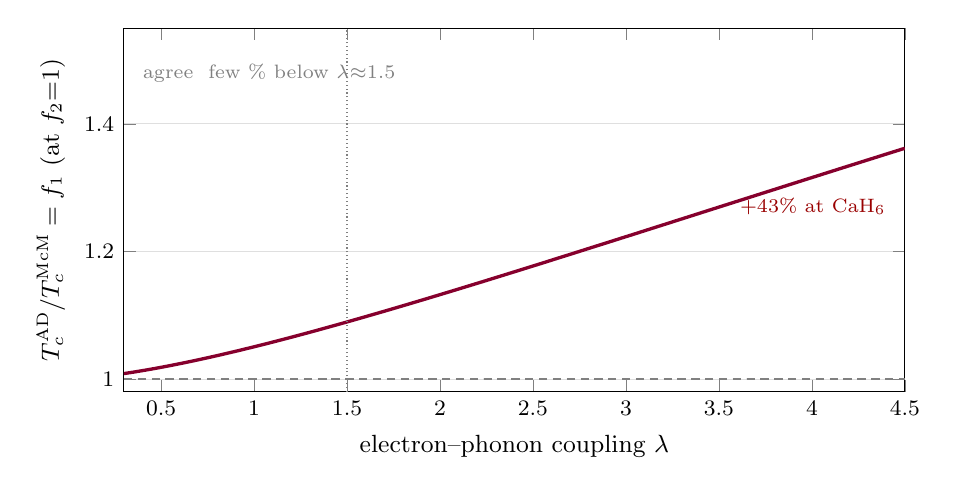
\begin{tikzpicture}
\begin{axis}[
  width=11.5cm, height=6.2cm,
  xlabel={electron--phonon coupling $\lambda$},
  ylabel={$T_c^{\mathrm{AD}}/T_c^{\mathrm{McM}}=f_1$ (at $f_2{=}1$)},
  xmin=0.3, xmax=4.5, ymin=0.98, ymax=1.55,
  tick label style={font=\footnotesize},
  label style={font=\small},
  ymajorgrids, grid style={gray!25},
  domain=0.3:4.5, samples=90,
]
\addplot[purple!70!black,very thick,smooth]
  {(1+(x/(2.46*(1+3.8*0.10)))^1.5)^(1/3)};
\addplot[gray,densely dashed,thick] {1};
% region annotations
\draw[gray,densely dotted] (axis cs:1.5,0.98) -- (axis cs:1.5,1.55);
\node[font=\scriptsize,gray,anchor=south west] at (axis cs:0.35,1.45)
  {agree $\lesssim$ few \% below $\lambda{\approx}1.5$};
\node[font=\scriptsize,red!60!black,anchor=north east] at (axis cs:4.45,1.30)
  {$+43$\% at CaH$_6$};
\end{axis}
\end{tikzpicture}
\caption{The McMillan$\to$Allen--Dynes correction ratio $f_1$ vs $\lambda$
($\mu^{*}=0.10$, $f_2{=}1$). The ratio is the formal statement of the
divergence charted in Fig.~\ref{fig:mcm-vs-ad}: $\approx\!1$ in the
conventional regime, growing to $+43$\% by the strong-coupling hydride
end. This is why the candidate slate of Appendix~\ref{app:hydride} is
ranked by Allen--Dynes, not McMillan.}
\label{fig:ad-vs-mcm-ratio}
\end{figure}

% -------------------------------------------------------------------------
\subsection{Honest scope}
\label{app:ad-honest}

Allen--Dynes is still a \emph{conventional} ($s$-wave, phonon-mediated)
closed form: it presumes Eliashberg theory holds, and like McMillan it is
exact only \emph{given} $(\lambda, \omega_{\log}, \bar\omega_2, \mu^{*})$
sourced from DFT (Appendix~\ref{app:elph}). It does not extend to $d$-wave
cuprates (the YBCO negative control of Appendix~\ref{app:material}), nor
does it predict dynamical stability or synthesizability. The
$|\Delta|=2.8\times10^{-11}$ on h3cl is a verification of the
\emph{kernel arithmetic}, not of h3cl's existence as a material. The
formula is \tierGreen; the \emph{material} stays \tierOrange\ and
\texttt{absorbed=false}. \textbf{No room-temperature superconductor is
claimed.}
